\section{Characterization of 3-planar graphs}
\label{sec:3planar}

%\todo[inline]{true planar subgraph or true planar skeleton?}
%\todo[inline]{change maximal to optimal}
Let $G$ be an optimal $3$-planar graph on $n$ vertices (and therefore with $5.5n-11$ edges) and let $\Gamma(G)$ be a PMCM $3$-planar drawing of $G$, i.e. $\Gamma(G)$ has the maximum number of true-planar edges among all potential $3$-planar drawing of $G$ and, subject to this restriction, $\Gamma(G)$ has also the minimum number of crossings. 
For the sake of simplicity we also assume that in the drawing $\Gamma(G)$ there is no pair of edges that cross twice, i.e. $\Gamma(G)$ is almost-simple. The assumption  will be settled  by Lemma~\ref{lem:3_planar_cross_twice}. In the following we examine structural properties of the almost-simple PMCM drawing $\Gamma(G)$, in particular we show  that the true planar skeleton$\Pi(G)$ of $\Gamma(G)$ consists of faces of length at most $9$. 
%The following lemmas describe some structural properties of $\Gamma(G)$.
%\todo[inline]{add in every lemma the assumption about edges crossing twice}


\begin{lemma}\label{lem:3_planar_true_planar}
Let $\Gamma(G)$ be a PMCM $3$-planar drawing of an optimal $3$-planar graph $G$ on $n$ vertices.
\begin{enumerate}
\item A true planar $6$-cycle in $\Gamma(G)$ without vertices in its interior, can not contain more than  $8$ chords in its interior; refer to Figure~\ref{fig:3_planar_polygon_conf_6}.
\item A true planar $7$-cycle in $\Gamma(G)$ without vertices in its interior, can not contain more than $9$ chords in its interior; refer to Figure~\ref{fig:3_planar_polygon_conf_7}.
\item A true planar $8$-cycle in $\Gamma(G)$ without vertices in its interior, can not contain more than $11$ chords in its interior; refer to Figure~\ref{fig:3_planar_polygon_conf_8}.
\item A true planar $9$-cycle in $\Gamma(G)$ without vertices in its interior, can not contain more than $14$ chords in its interior; refer to Figure~\ref{fig:3_planar_polygon_conf_9}.
\item A true planar $10$-cycle in $\Gamma(G)$ without vertices in its interior, can not contain more than $17$ chords in its interior; refer to Figure~\ref{fig:3_planar_polygon_conf_10}.
\item A $7$-cycle in $\Gamma(G)$ with exactly one edge crossing its boundary can contain at least $10$ edges: $9$ chords in its interior  and an edge that crosses its boundary (with one crossing); refer to Figure~\ref{fig:3_planar_polygon_conf_7_stick}.
\item A $8$-cycle in $\Gamma(G)$ with exactly one edge crossing its boundary can contain at least $12$ edges: $11$ chords in its interior and an edge that crosses its boundary (with two crossings); refer to Figure~\ref{fig:3_planar_polygon_conf_8_stick}.
\end{enumerate}
\end{lemma}
\begin{proof}
The proof of this lemma is omitted as it can be checked exhaustively.
\end{proof}

\begin{figure}[htb]
    \centering
    \begin{minipage}[b]{.24\textwidth}
        \centering
        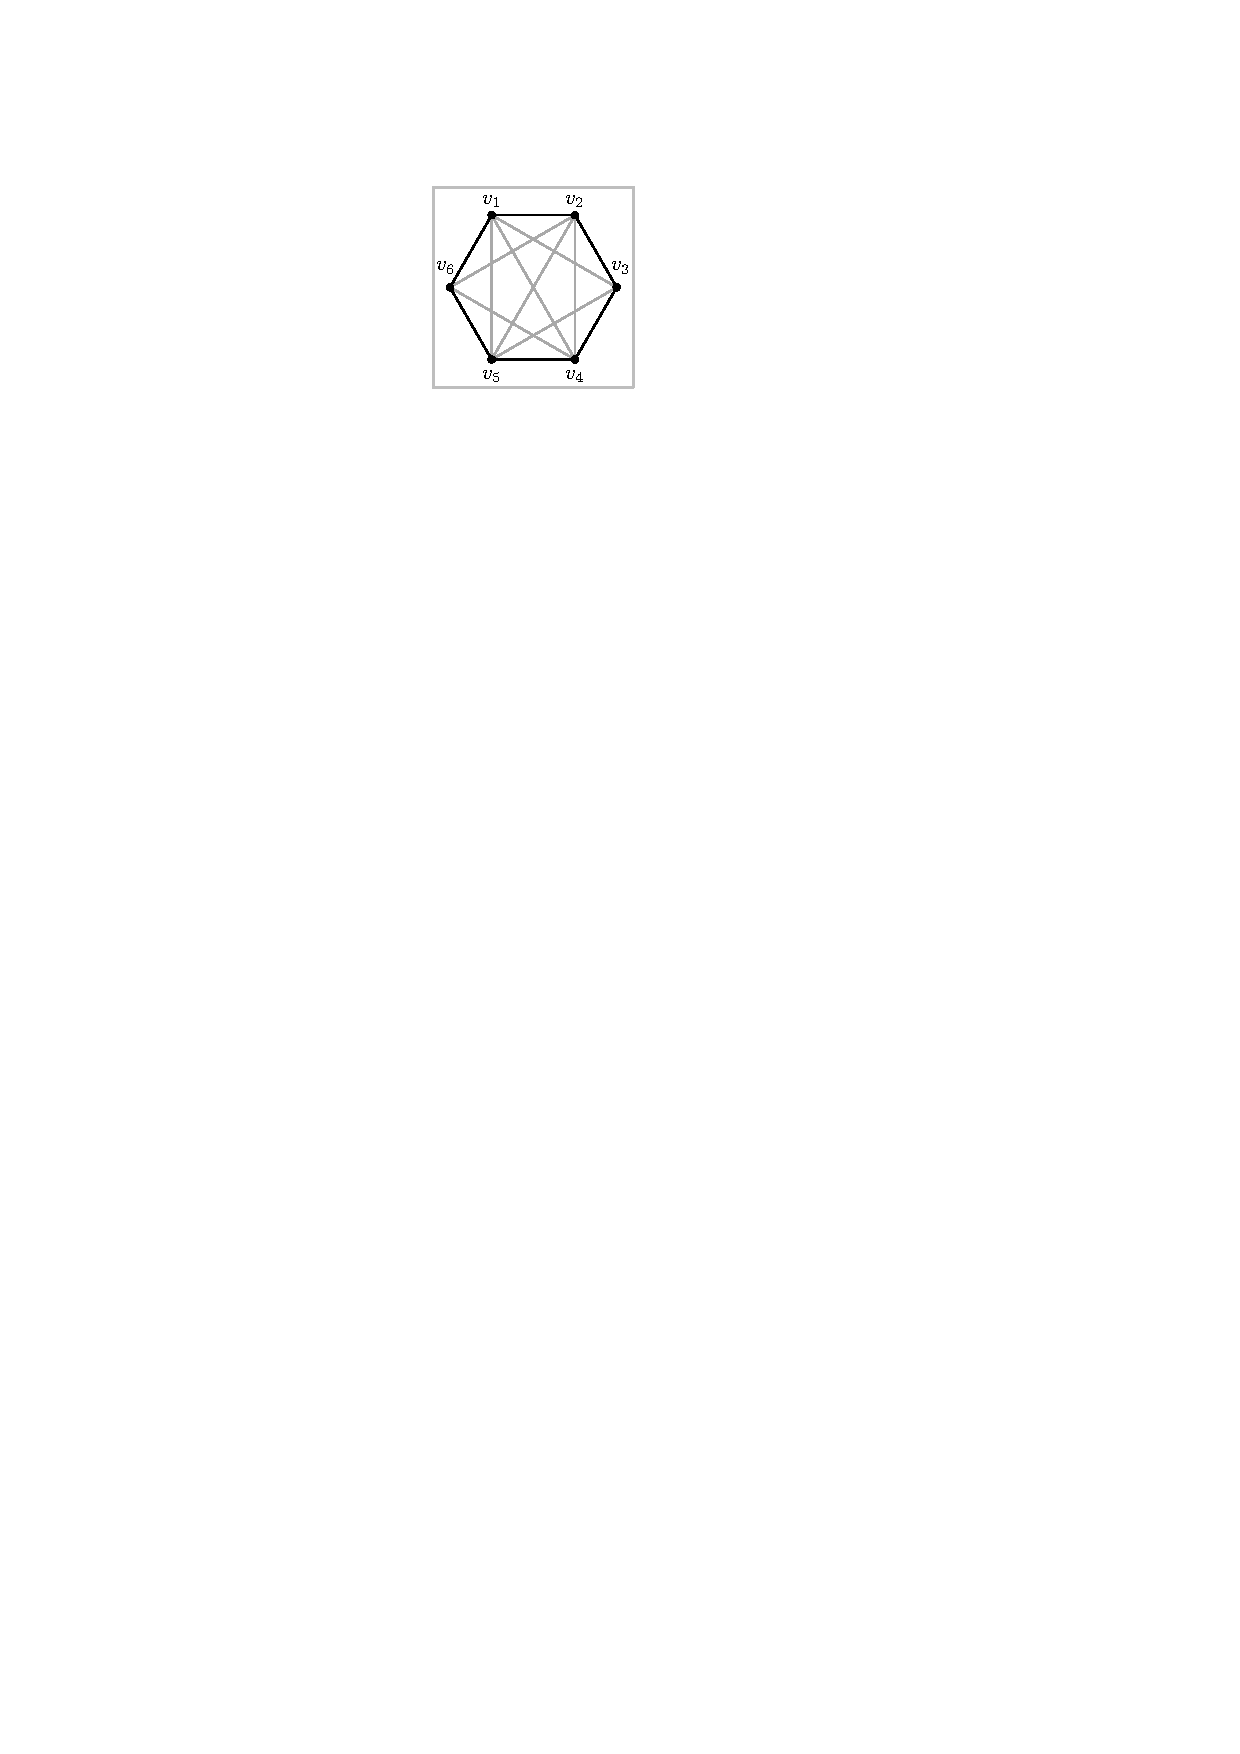
\includegraphics[width=\textwidth,page=1]{images/polygon_conf}
        \subcaption{~}\label{fig:3_planar_polygon_conf_6}
    \end{minipage}
    \begin{minipage}[b]{.24\textwidth}
        \centering
        \includegraphics[width=\textwidth,page=2]{images/polygon_conf}
        \subcaption{~}\label{fig:3_planar_polygon_conf_7}
    \end{minipage}
    \begin{minipage}[b]{.24\textwidth}
        \centering
        \includegraphics[width=\textwidth,page=3]{images/polygon_conf}
        \subcaption{~}\label{fig:3_planar_polygon_conf_8}
    \end{minipage}
    \begin{minipage}[b]{.24\textwidth}
        \centering
        \includegraphics[width=\textwidth,page=4]{images/polygon_conf}
        \subcaption{~}\label{fig:3_planar_polygon_conf_9}
    \end{minipage}
    \begin{minipage}[b]{.24\textwidth}
        \centering
        \includegraphics[width=\textwidth,page=5]{images/polygon_conf}
        \subcaption{~}\label{fig:3_planar_polygon_conf_10}
    \end{minipage}
		\begin{minipage}[b]{.24\textwidth}
        \centering
        \includegraphics[width=\textwidth,page=6]{images/polygon_conf}
        \subcaption{~}\label{fig:3_planar_polygon_conf_7_stick}
    \end{minipage}
    \begin{minipage}[b]{.24\textwidth}
        \centering
        \includegraphics[width=\textwidth,page=7]{images/polygon_conf}
        \subcaption{~}\label{fig:3_planar_polygon_conf_8_stick}
    \end{minipage}
    \caption{%
    Configurations of Lemma~\ref{lem:3_planar_true_planar}.
    \label{fig:3_planar_polygon_conf}}
\end{figure}

Denote by $m_P(k)$ be the maximum number of chords in a true planar $k$-cycle (without vertices in its interior) of the drawing $\Gamma(G)$ as given by Lemma~\ref{lem:3_planar_true_planar}, for $6\leq k\leq 10$. 

\begin{lemma}\label{lem:3_planar_polygon}
Let $\Gamma(G)$ be a PMCM $3$-planar drawing of an optimal $3$-planar graph $G$ on $n$ vertices, and let $k$ such that $6\leq k\leq 9$. Suppose that there exists a \pp $\mathcal{P}_k$ of $k$ vertices in $\Gamma(G)$, such that the boundary edges of $\mathcal{P}_k$ exist in the drawing. Let $E_k$ be the set of edge-segments that pass through $\mathcal{R}_k$, and $m_k=|E_k|$.If: 
\begin{enumerate}
\item $m_k\leq 2k-4$, and, 
\item every edge-segment of $E_k$ has at least one crossing in $\mathcal{R}_k$,
\end{enumerate}
%\todo{replace every edge with every part of any edge}
then there exists a true planar $k'$-cycle in $\Gamma(G)$ (without vertices in its interior), with $k\leq k'\leq 9$, with all edge-segments of $E_k$ as chords.
\end{lemma}

\begin{proof}
Before proving the lemma we need to make the following remark: \todo{perhaps rephrase if not clear}If an edge-segment of an edge $e$ belongs to $E_k$ then no other edge-segment of $e$ lies inside $\mathcal{R}_k$. This is true, since if at least two edge-segments of $e$ lie inside $\mathcal{R}_k$, then each edge-segment has at least one crossing in $\mathcal{R}_k$ (by the assumptions of the lemma) and at least one crossing with the boundary of $\mathcal{P}_k$ (otherwise there would be only one edge-segment of $e$ in $E_k$). Hence, $e$ has at least $4$ crossings in $\Gamma(G)$ which is not allowed. 
 
First, we prove the lemma for the case $k=9$. Let $C$ be the $9$-cycle defined by the boundary of the \pp $\mathcal{P}$, with vertices $v_1,v_2,\dots,v_9$, and let $E$ the set of edge-segments that pass through its \pr $\mathcal{R}$ and apply to the conditions of the lemma. If no edge with edge-segment in $E$ crosses an edge of $C$,  then $C$ is clearly a true planar $9$-cycle, and the lemma holds for $k'=k$. So, suppose that at least one edge with edge-segment in $E$, say $e$ crosses an edge of $C$ (refer to Figure~\ref{fig:3_planar_polygon_before}). W.l.o.g. we can assume that $e$ crosses edge $(v_1,v_2)$ of $C$. Let $c$ be the crossing point of $e$ and $(v_1,v_2)$. If $w$ and $w'$ are the two endpoints of $e$, we have that either edge-segment $(w,c)$ of $e$ or edge-segment $(c,w')$ of $e$ is entirely drawn outside $\mathcal{R}$ (otherwise $e$ would have at least two edge-segments in $E$, which is not possible as explained earlier). Assume w.l.o.g. that  $(w,c)$ part of $e$ is drawn outside $\mathcal{R}$. Then \pes $[v_1,w]$ and $[w,v_2]$ are corner edges. Note that $e$ has already at least two crossings: one in $\mathcal{R}$ (assumption of the lemma) and one with edge $(v_1,v_2)$. This implies that there exists at most one edge, say $e'$ (where $e'$ might have an edge-segment in $E$ or not), crossing with $e$. Vertices $v_1,w,v_2,\dots,v_9$ define a \pp $\mathcal{P}'$ on $10$ vertices (see Figure~\ref{fig:3_planar_polygon_after}) and, for the set of edge-segments $E'$ that pass through its \pr $\mathcal{R}'$, we have that $E'$ contains all edge-segments of $E$ plus at most two more: the open edge-segment defined by $(v_1,v_2)$, and possibly an edge-segment of $e'$. Hence $E'$ defines at most  $16$ edges. However, by Lemma~\ref{lem:3_planar_true_planar}, we can replace $E'$ with a $3$-planar pattern that defines $17$ edges (refer to Figure~\ref{fig:3_planar_polygon_conf_10}). The derived graph has more edges that $G$, a contradiction to the optimality of $G$. Hence we have concluded that for $k=9$, $C$ is a true planar cycle on $9$ vertices.

%First, we prove the lemma for the case $k=9$. Let $C$ be the $9$-cycle defined by the boundary of the \pp $\mathcal{P}$, with vertices $v_1,v_2,\dots,v_9$, and let $E$ the set of edge-segments that pass through its polygonal region $\mathcal{R}$ and apply to the conditions of the lemma. If no edge of $E$ crosses an edge of $C$,  then $C$ is clearly a true planar $9$-cycle, and the lemma holds for $k'=k$. So, suppose that at least one edge, say $e$ crosses an edge of $C$ (refer to Figure~\ref{fig:3_planar_polygon_before}). W.l.o.g. we can assume that $e$ crosses edge $(v_1,v_2)$ of $C$. Let $c$ be the crossing point of $e$ and $(v_1,v_2)$. If $w$ and $w'$ are the two endpoints of $e$, we have that either $(w,c)$ part of $e$ or $(c,w')$ part of $e$ is entirely drawn outside $\mathcal{R}$ (refer to above remark). Assume w.l.o.g. that  $(w,c)$ part of $e$ is drawn outside $\mathcal{R}$. Then edges $(v_1,w)$ and $(w,v_2)$ are potential corner edges. Note that $e$ has already at least two crossings: one in $\mathcal{R}$ (assumption of the lemma) and one with edge $(v_1,v_2)$. This implies that there exists at most one edge, say $e'$, where $e'\notin E$, crossing with $e$. Vertices $v_1,w,v_2,\dots,v_9$ define a \pp $\mathcal{P}'$ on $10$ vertices (see Figure~\ref{fig:3_planar_polygon_after}) and, for the set of edges $E'$ that pass through its polygonal region $\mathcal{R}'$, we have that $E'=E\cup\left\{(v_1,v_2), e'\right\}$, and $|E'|\leq 16$. However, by Lemma~\ref{lem:3_planar_true_planar}, we can replace $E'$ with a $3$-planar pattern that has $17$ edges (refer to Figure~\ref{fig:3_planar_polygon_conf_10}). The derived graph has more edges that $G$, a contradiction to the optimality of $G$. Hence we have concluded that for $k=9$, $C$ is a true planar cycle on $9$ vertices.

Now, for the rest of the cases, assume that the lemma holds for $6<k\leq 9$. We will prove that it also holds for $k-1$. So, let $C$ be a $k-1$-cycle defined by the boundary of a \pp $\mathcal{P}$, with vertices $v_1,v_2,\dots,v_{k-1}$, and let $E$ the set of edge-segments that pass through its \pr $\mathcal{R}$ and apply to the conditions of the lemma. As in the previous case, if no edge with edge-segment in $E$ crosses an edge of $C$,  then $C$ is clearly a true planar $k-1$-cycle, and the lemma holds for $k'=k-1$. So, suppose that at least one edge with edge-segment in $E$, say $e$ crosses an edge of $C$. W.l.o.g. we can assume that $e$ crosses edge $(v_1,v_2)$ of $C$. Let $c$ be the crossing point of $e$ and $(v_1,v_2)$. If $w$ and $w'$ are the two endpoints of $e$, we have that either edge-segment $(w,c)$ of $e$ or edge-segment $(c,w')$ of $e$ is entirely drawn outside $\mathcal{R}$. Assume w.l.o.g. that edge-segment $(w,c)$ of $e$ is drawn outside $\mathcal{R}$. Then \pes $[v_1,w]$ and $[w,v_2]$ are corner edges. Note that $e$ has already at least two crossings: one in $\mathcal{R}$ (assumption of the lemma) and one with edge $(v_1,v_2)$. This implies that there exists at most one edge, say $e'$ (where $e'$ might have an edge-segment in $E$ or not), crossing with $e$. Vertices $v_1,w,v_2,\dots,v_{k-1}$ define a \pp $\mathcal{P}'$ on $k$ vertices and, for the set of edge-segments $E'$ that pass through its polygonal region $\mathcal{R}'$, we have that contains all edge-segments of $E$ plus at most two more: the open edge-segment defined by $(v_1,v_2)$, and possibly an edge-segment of $e'$. Hence $|E'|\leq 2k-4$. However, by Lemma~\ref{lem:3_planar_true_planar}, we can replace $E'$ with a $3$-planar pattern that has $2k-4$ edges (refer to Figures~\ref{fig:3_planar_polygon_conf_7_stick}, \ref{fig:3_planar_polygon_conf_8_stick}, \ref{fig:3_planar_polygon_conf_9} for $k=7,8,9$ resp.). Since $G$ is optimal, the derived graph has the same number of edges as $G$. This can only be true if all boundary edges of $\mathcal{P}'$ exist in $\Gamma(G)$. Then, the vertices of $\mathcal{P}'$ define a $k$-cycle in $\Gamma(G)$ that satisfies the assumptions of the lemma: $|E'|=2k-4$ and every edge-segment of $E'$ has at least one crossing in $\mathcal{R}'$ (this is true for all edge-segments of $E\subset E'$ and also for the edge-segments of $(v_1,v_2)$ and $e'$ since they cross $e$ in the interior of $\mathcal{R}'$). By the induction hypothesis, there exists a true planar cycle on $k'$ vertices, where $k\leq k'\leq 9$, with all edge-segments of $E'$, and therefore of $E$,  as chords.


%Now, for the rest of the cases, assume that the lemma holds for $6<k\leq 9$. We will prove that it also holds for $k-1$. So, let $C$ be a $k-1$-cycle defined by the boundary of a \pp $\mathcal{P}$, with vertices $v_1,v_2,\dots,v_{k-1}$, and let $E$ the set of edge-segments that pass through its polygonal region $\mathcal{R}$\todo{and apply to the conditions of the lemma}. As in the previous case, if no edge of $E$ crosses an edge of $C$,  then $C$ is clearly a true planar $k-1$-cycle, and the lemma holds for $k'=k$. So, suppose that at least one edge, say $e$ crosses an edge of $C$. W.l.o.g. we can assume that $e$ crosses edge $(v_1,v_2)$ of $C$. Let $c$ be the crossing point of $e$ and $(v_1,v_2)$. If $w$ and $w'$ are the two endpoints of $e$, we have that either $(w,c)$ part of $e$ or $(c,w')$ part of $e$ is entirely drawn outside $\mathcal{R}$. Assume w.l.o.g. that  $(w,c)$ part of $e$ is drawn outside $\mathcal{R}$. Then edges $(v_1,w)$ and $(w,v_2)$ are potential corner edges. Note that $e$ has already at least two crossings: one in $\mathcal{R}$ (assumption of the lemma) and one with edge $(v_1,v_2)$. This implies that there exists at most one edge, say $e'$, where $e'\notin E$, crossing with $e$. Vertices $v_1,w,v_2,\dots,v_{k-1}$ define a \pp $\mathcal{P}'$ on $k$ vertices and, for the set of edges $E'$ that pass through its polygonal region $\mathcal{R}'$, we have that $E'=E\cup\left\{(v_1,v_2), e'\right\}$, and $|E'|\leq 2k-4$. However, by Lemma~\ref{lem:3_planar_true_planar}, we can replace $E'$ with a $3$-planar pattern that has $2k-4$ edges (refer to Figures~\ref{fig:3_planar_polygon_conf_7_stick}, \ref{fig:3_planar_polygon_conf_8_stick}, \ref{fig:3_planar_polygon_conf_9} for $k=7,8,9$ resp.). Since $G$ is optimal, the derived graph has the same number of edges as $G$. This can only be true if all boundary edges of $\mathcal{P}'$ exist in $\Gamma(G)$. Then, the vertices of $\mathcal{P}'$ define a $k$-cycle in $\Gamma(G)$ that satisfies the assumptions of the lemma: $|E'|=2k-4$ and every edge\todo{every part of any edge } of $E'$ has at least one crossing in $\mathcal{R}'$ (this is true for all edges of $E\subset E'$ and also for edges $(v_1,v_2)$ and $e'$ since their crossing point $c$ is in the interior of $\mathcal{R}'$). Then there exists a true planar cycle on $k\leq k'\leq 9$ vertices with all edges of $E'$, and therefore of $E$,  as chords.\qed
\end{proof}

%\todo[inline]{move the definition}
Suppose that in a PMCM drawing $\Gamma(G)$ an edge $e$ is crossed by two edges $e_1$ and $e_2$, where $e_i=(u_i,v_i)$ for $i=1,2$. Recall that if $\Gamma(G)$ is almost-simple then at least one of parallel edges $[u_1,u_2]$ and $[v_1,v_2]$ is a \pe of $\Gamma(G)$. Also, in the case where both parallel edges $[u_1,u_2]$ and $[v_1,v_2]$ are \pes of $\Gamma(G)$, $e_1$ and $e_2$ are called independent.

\begin{lemma}\label{lem:3_planar_independent}
Let $\Gamma(G)$ be an almost-simple PMCM $3$-planar drawing of an optimal $3$-planar graph $G$ on $n$ vertices. If an edge is crossed by two independent edges, then it is a chord of a true planar $k$-cycle (without vertices in its interior), with $6\leq k\leq 9$.
\end{lemma}
\begin{proof}
Let $e=(u,v)$ be an edge of $\Gamma(G)$ that crosses with  $e_1$ and $e_2$, where $e_i=(u_i,v_i)$ for $i=1,2$. Since $e_1$ and $e_2$ are independent edges, both parallel edges $[u_1,u_2]$ and $[v_1,v_2]$ are \pes, as in Figure~\ref{fig:3_planar_independent}. Then vertices $u,u_1,u_2,v,v_2,v_1$ define a \pp $\mathcal{P}_6$ of six vertices (grey shaded in Figure~\ref{fig:3_planar_independent}). The \pr $\mathcal{R}_6$ of $\mathcal{P}_6$ contains no vertices in its interior, and at most $8$ edges of $\Gamma(G)$ define edge-segments that pass through $\mathcal{R}_6$: edges $(u,v)$, $(u_1,v_1)$, $(u_2,v_2)$, at most one other edge that crosses $(u,v)$, and at most four other edges that cross $(u_1,v_1)$ or $(u_2,v_2)$. We proceed by removing  edges $(u,v)$, $(u_1,v_1)$, $(u_2,v_2)$ and all other edges that cross $(u,v)$, $(u_1,v_1)$ or $(u_2,v_2)$, and replace them with the $3$-planar pattern of Figure~\ref{fig:3_planar_polygon_conf_6}. In the derived graph there exist $8$ edges drawn in $\mathcal{R}_6$ and do not cross the boundary of the \pp. Since $G$ is optimal, all boundary edges of $\mathcal{P}_6$ already exist in $\Gamma(G)$. Furthermore, all edge-segments that pass through $\mathcal{R}_6$ have at least one crossing in $\mathcal{R}_6$. Then, we can apply Lemma~\ref{lem:3_planar_polygon}, and conclude that there exists a true planar $k$-cycle without vertices in its interior ($6\leq k\leq 9$), that contains $e$ as a chord.
\end{proof}

%\begin{lemma}\label{lem:3_planar_independent}
%Let $\Gamma(G)$ be a $3$-planar drawing of an optimal $3$-planar graph $G$ on $n$ vertices. If an edge is crossed by two independent parallel edges, then it is a chord of a true planar $k$-cycle (without vertices in its interior), with $6\leq k\leq 9$.
%\end{lemma}
%\begin{proof}
%Let $e=(u,v)$ be an edge of $\Gamma(G)$ that crosses with  $e_1$ and $e_2$, where $e_i=(u_i,v_i)$ for $i=1,2$. Since $e_1$ and $e_2$ are independent parallel edges, both potential parallel edges $(u_1,u_2)$ and $(v_1,v_2)$ exist, as in Figure~\ref{fig:3_planar_independent}. Then vertices $u,u_1,u_2,v,v_2,v_1$ define a \pp $\mathcal{P}_6$ of six vertices (grey shaded in Figure~\ref{fig:3_planar_independent}). The polygonal region $\mathcal{R}_6$ of $\mathcal{P}_6$ contains no vertices in its interior, and at most $8$ edges of $\Gamma(G)$ pass through $\mathcal{R}_6$: edges $(u,v)$, $(u_1,v_1)$, $(u_2,v_2)$, at most one other edge that crosses $(u,v)$, and at most four other edges that cross $(u_1,v_1)$ or $(u_2,v_2)$. We proceed by removing  edges $(u,v)$, $(u_1,v_1)$, $(u_2,v_2)$ and all other edges that cross $(u,v)$, $(u_1,v_1)$ or $(u_2,v_2)$, and replace them with the $3$-planar pattern of Figure~\ref{fig:3_planar_polygon_conf_6}. In the derived graph there exist $8$ edges drawn in $\mathcal{R}_6$ and do not cross the boundary of the \pp. Since $G$ is optimal, all boundary edges of $\mathcal{P}_6$ already exist in $\Gamma(G)$. Then, we can apply Lemma~\ref{lem:3_planar_polygon}, and conclude that there exists a true planar $k$-cycle without vertices in its interior ($6\leq k\leq 9$), that contains $e$ as a chord.\qed
%\end{proof}

\begin{figure}[htb]
    \centering
    \begin{minipage}[b]{.24\textwidth}
        \centering
        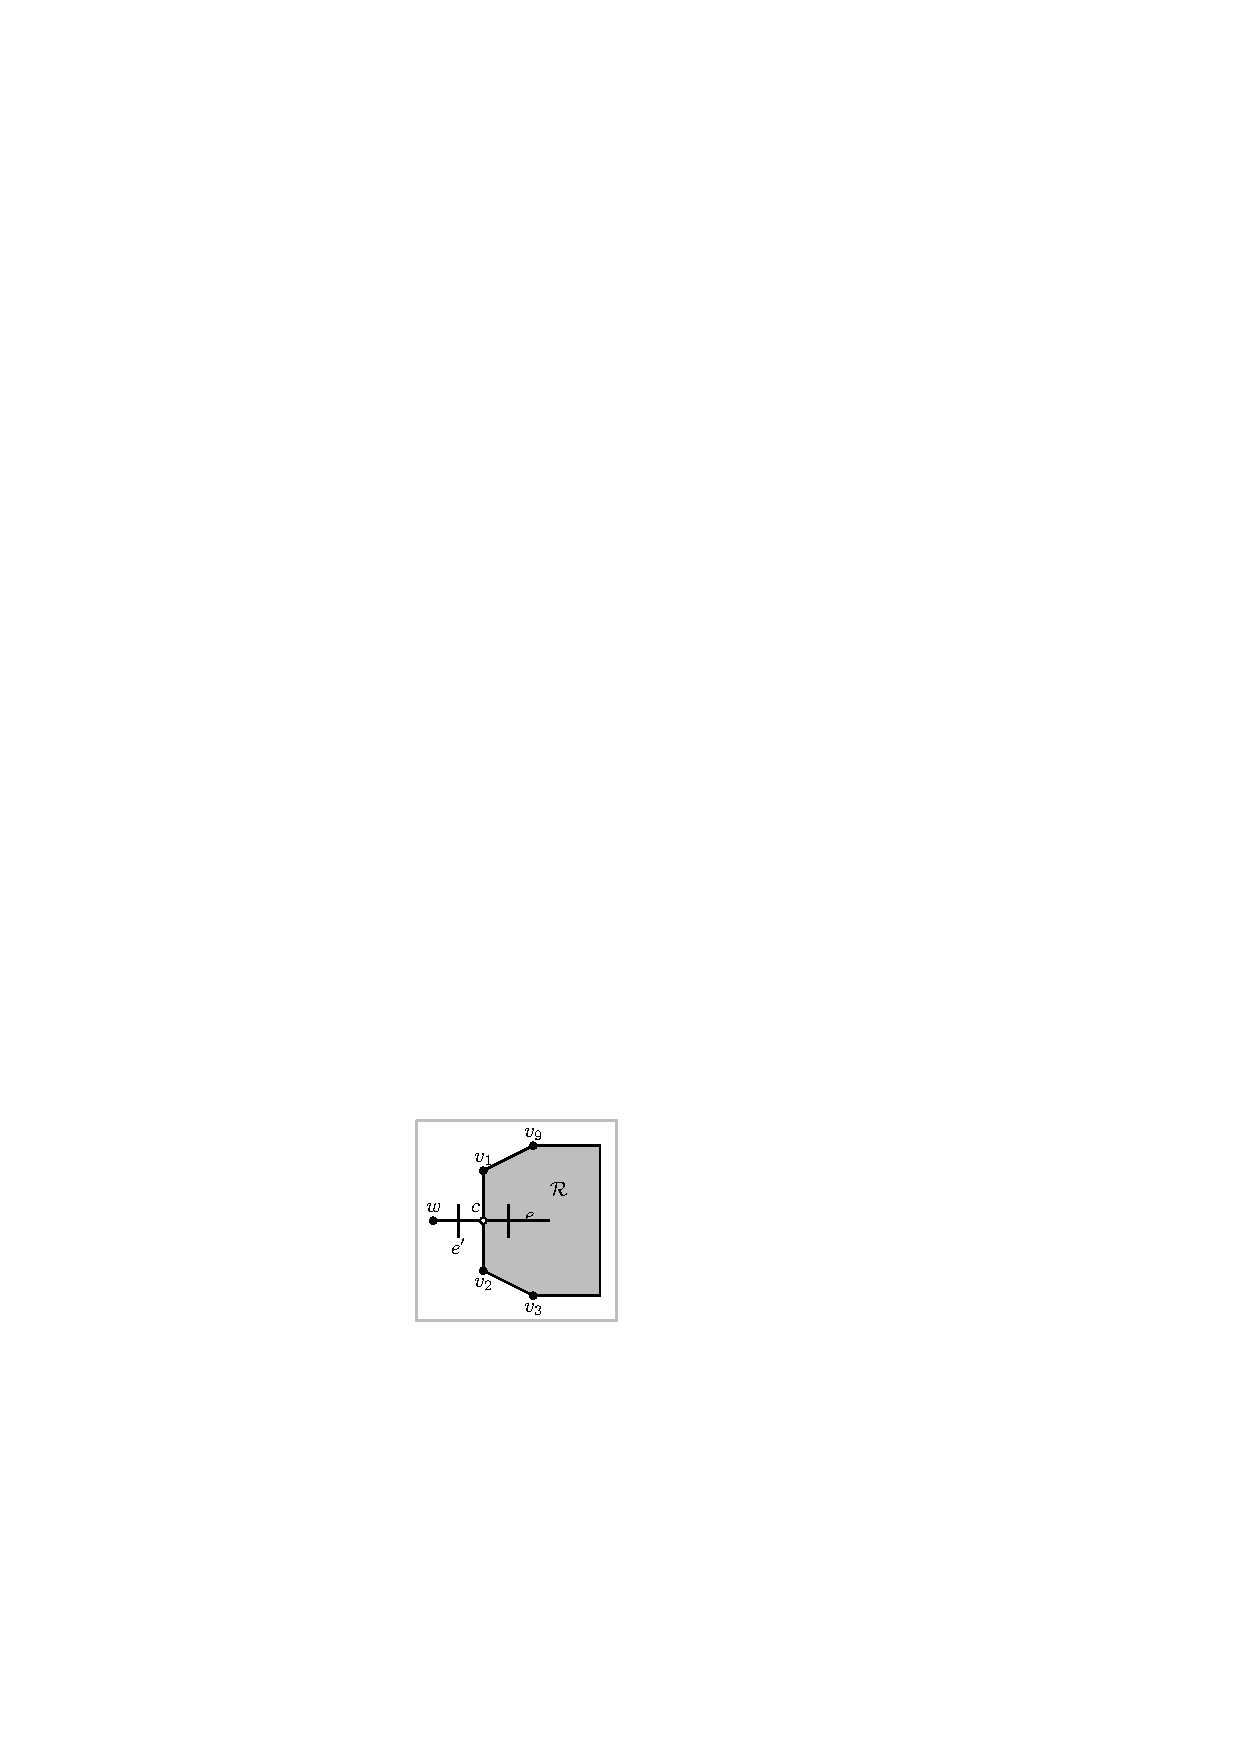
\includegraphics[width=\textwidth,page=1]{images/3planar_polygon}
        \subcaption{~}\label{fig:3_planar_polygon_before}
    \end{minipage}
    \begin{minipage}[b]{.24\textwidth}
        \centering
        \includegraphics[width=\textwidth,page=2]{images/3planar_polygon}
        \subcaption{~}\label{fig:3_planar_polygon_after}
    \end{minipage}
    \begin{minipage}[b]{.24\textwidth}
        \centering
        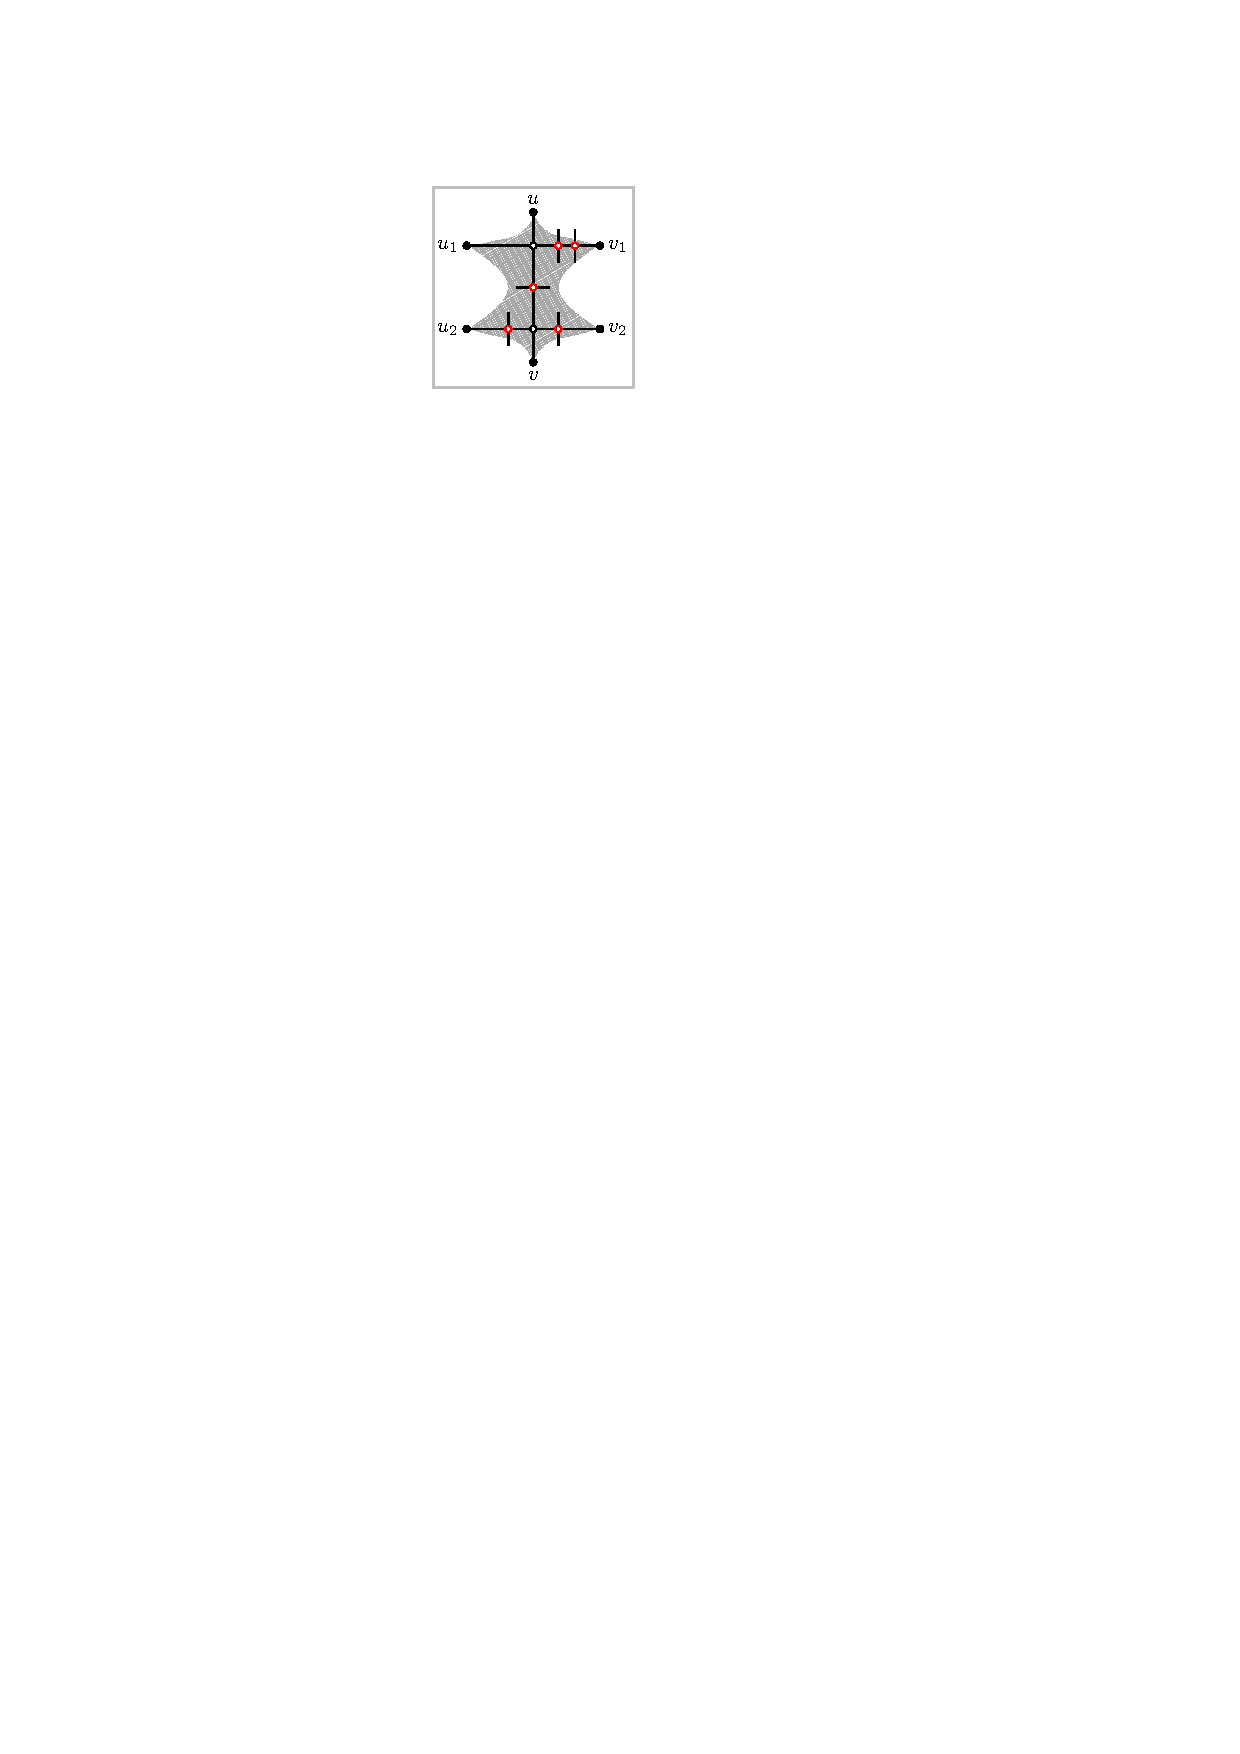
\includegraphics[width=\textwidth,page=1]{images/3planar_independent}
        \subcaption{~}\label{fig:3_planar_independent}
    \end{minipage}
    \caption{%
    (a)-(b):~Configurations of Lemma~\ref{lem:3_planar_polygon}, (c):~Configuration of Lemma~\ref{lem:3_planar_independent}}.
    \label{fig:3_planar_polygon}
\end{figure}


\todo[inline]{move the definition}
Consider the so called crossing graph $G_C$ of the drawing $\Gamma(G)$. The vertices of $G_C$ correspond to the edges of $G$ and two vertices of $G_C$ are adjacent if and only if the corresponding edges of $G$ cross in $\Gamma(G)$. The connected components of $G_C$ define a partition of the edges $E(G)$ of $G$ to \emph{propagated sets of crossing edges}. If $e\in E(G)$ we denote by $S(e)$ the unique propagated set of crossing edges that $e$ belongs to. Note that if $e$ is a chord of a true planar $k$-cycle in the drawing $\Gamma(G)$ that has no vertices in its interior, then all edges of $S(e)$ are also chords of the $k$-cycle.

Now we are ready to state the main property of almost-simple PMCM-drawings of optimal $3$-planar  graphs:

\begin{lemma}\label{lem:3_planar_small_faces}
Let $\Gamma(G)$ be an almost-simple PMCM $3$-planar drawing of an optimal $3$-planar graph $G$ on $n$ vertices. Any edge that is crossed three times in  $\Gamma(G)$ is a chord of a true-planar $k$-cycle in $\Gamma(G)$ (without vertices in its interior), where $6\leq k\leq 9$. 
\end{lemma}

\begin{proof}
Let $e=(u,v)$ be an edge of $G$ that crosses with edges $e_i=(u_i,v_i)$ in $\Gamma(G)$, for $i=1,2,3$. Consider the propagated set of crossing edges $S(e)$ where $e$ belongs to. We distinguish two cases depending on whether there exists an edge in $S(e)$ that crosses with two independent edges or not.

Suppose that this is the case, and an edge of $S(e)$ is crossed by two independent edges. Then by Lemma~\ref{lem:3_planar_independent}, there exists a true planar $k$-cycle (without vertices in its interior) defining a \pr with this edge as a chord. Then all edges of $S(e)$ are also drawn as chords of the $k$-cycle and the lemma follows.

Assume, now that all edges of $S(e)$ with at least two crossings, are not crossed by independent edges in $\Gamma(G)$. Then, for edge $e$, that crosses with edges $e_1$, $e_2$, and $e_3$, we have that edges $e_i$, $e_j$ ($1\leq i<j\leq 3$) are not parallel edges. This implies that exactly one of parallel edges $[u_i,u_j]$ or $[v_i,v_j]$ is not a \pe. For the sake of simplicity let's refer to parallel edges $[u_i,u_j]$ and $[v_i,v_j]$ as the ``$u$-parallel edge'' and ``$v$-parallel edge'' respectively of $e_i$ and $e_j$. 
There are three ways to combine indices $i$ and $j$ and for every combination exactly one of the ``$u$-parallel edge'' and ``$v$-parallel edge'' is not a \pe. This implies that: there exist at least two combinations such that their ``$u$-parallel edges'' are not \pes, or there exist at least two combinations such that their ``$v$-parallel edges'' are not \pes of $\Gamma(G)$. W.l.o.g. assume that there exist two combinations of indices, say $i_1$ with $j_1$ and $i_2$ with $j_2$ for which their ``$u$-parallel edges'', namely $[u_{i_1},u_{j_1}]$ and $[u_{i_2},u_{j_2}]$  are not \pes. It is clear that since $i_1\neq j_1$, $i_2\neq j_2$ and $\left\{i_1,i_2,j_1,j_2\right\}\subset\left\{1,2,3\right\}$, at least two indices are the same. W.l.o.g. assume that $i_1=i_2$; other cases are symmetric. Let$i=i_1=i_2$. Then we have that parallel edges  $(u_i,u_{j_1})$ and $(u_i,u_{j_2})$ are not \pes, where $j_1\neq j_2$. This implies that $u_i=u_{j_1}$ and $u_i=u_{j_2}$. It is not hard to see that parallel edge $(u_{j_1},u_{j_2})$ can not be a \pe either; for an example refer to Figure~\ref{fig:3_planar_small_faces_example}, where $i=1$. Hence, for any edge of $S(e)$ with three crossings in $\Gamma(G)$, we have the crossing pattern of Figure~\ref{fig:3_planar_small_faces_conf}, where the grey-shaded region has no vertices in its interior.

%Since there are three pairs of potential parallel edges $e_i$ and $e_j$, there exist at least two pairs, say $e_i$-$e_j$ and $e_{i'}$-$e_{j'}$ for which both \pes $(u_i,u_j)$ and $(u_{i'},u_{j'})$, or both \pes $(v_i,v_j)$ and $(v_{i'},v_{j'})$ do not exist. Assume w.l.o.g. that edges $(u_i,u_j)$ and $(u_{i'},u_{j'})$ do not exist. Since $1\leq i,i',j,j'\leq 3$ and $i\neq j$, $i'\neq j'$, we can also assume that $i=i'$. Then we have that potential parallel edges  $(u_i,u_j)$ and $(u_i,u_{j'})$ do not exist. This implies that $u_i=u_j$ and $u_i=u_j'$. Also, the potential parallel edge $(u_j,u_{j'})$ can not exist, since otherwise at least one of potential parallel edges $(u_i,u_j)$ or $(u_i,u_{j'})$ would also exist (for an example refer to Figure~\ref{fig:3_planar_small_faces_example}, where $i=1$). Hence, for any edge of $S(e)$ with three crossings in $\Gamma(G)$, we have the crossing pattern of Figure~\ref{fig:3_planar_small_faces_conf}, where the grey-shaded region has no vertices in its interior.

So far, vertices $u,v_1,v_2,v_3,v,u_1$ define a \pp $\mathcal{P}$ on six vertices. We want to apply Lemma~\ref{lem:3_planar_polygon} for $k=6$, and to achieve this, we claim that there exist at most $8$ edges that pass through the \pr $\mathcal{R}$ of $\mathcal{P}$ and satisfy the lemma requirements, and also that all boundary edges of $\mathcal{P}$ exist in $\Gamma(G)$. So, suppose that there exists an edge $e'=(u',v')$ that crosses with $e_2$ in the interior of $\mathcal{R}$. Since $e_2\in S(e)$, $e_2$ is not crossed by independent edges. So, edges $e'=(u',v')$ and $e=(u,v)$ are not independent edges, and exactly one of parallel edges $[u,u']$ or $[v,v']$ is not a \pe. Assume w.l.o.g. that parallel edge $[u,u']$ is not a \pe. This implies that $u=u'$ and that the region $R$ defined by edges $e_2$, $e$ and $e'$ has no vertices in its interior (see Figure~\ref{fig:3_planar_small_faces_conf_middle_a}). Then, $e'$ must cross with $e_1$, as otherwise vertex $v_1$ would be in the interior of $R$; refer to Figure~\ref{fig:3_planar_small_faces_conf_middle_b}. Hence, any edge that crosses with $e_2$, must also cross with $e_1$ or $e_3$. Then, there exist at most four other edges that pass through the polygonal region $\mathcal{R}$ and cross with edges $e_1$, $e_2$ or $e_3$, i.e. we have at most $8$ edges that pass through $\mathcal{R}$. We proceed by removing edges $e$, $e_i$ and all edges that cross with edges $e_i$ in  $\mathcal{R}$ ($i=1,2,3$), and replace them with the $3$-planar pattern of Figure~\ref{fig:3_planar_polygon_conf_6}. The derived graph has at least as many edges as $G$, and since $G$ is optimal, the boundary edges of $\mathcal{P}$ exist in the drawing $\Gamma(G)$. So, the vertices of $\mathcal{P}$ define a $6$-cycle in $\Gamma(G)$ (without vertices in its interior), with $8=2*6-4$ edge-segments passing through $\mathcal{R}$, and these edge-segments have at least one crossing inside $\mathcal{R}$. By Lemma~\ref{lem:3_planar_polygon}, for $k=6$, we have that $e$ is a chord of a true planar $k'$-cycle for $6\leq k'\leq 9$.
\end{proof}

\begin{figure}[htb]
    \centering
    \begin{minipage}[b]{.24\textwidth}
        \centering
        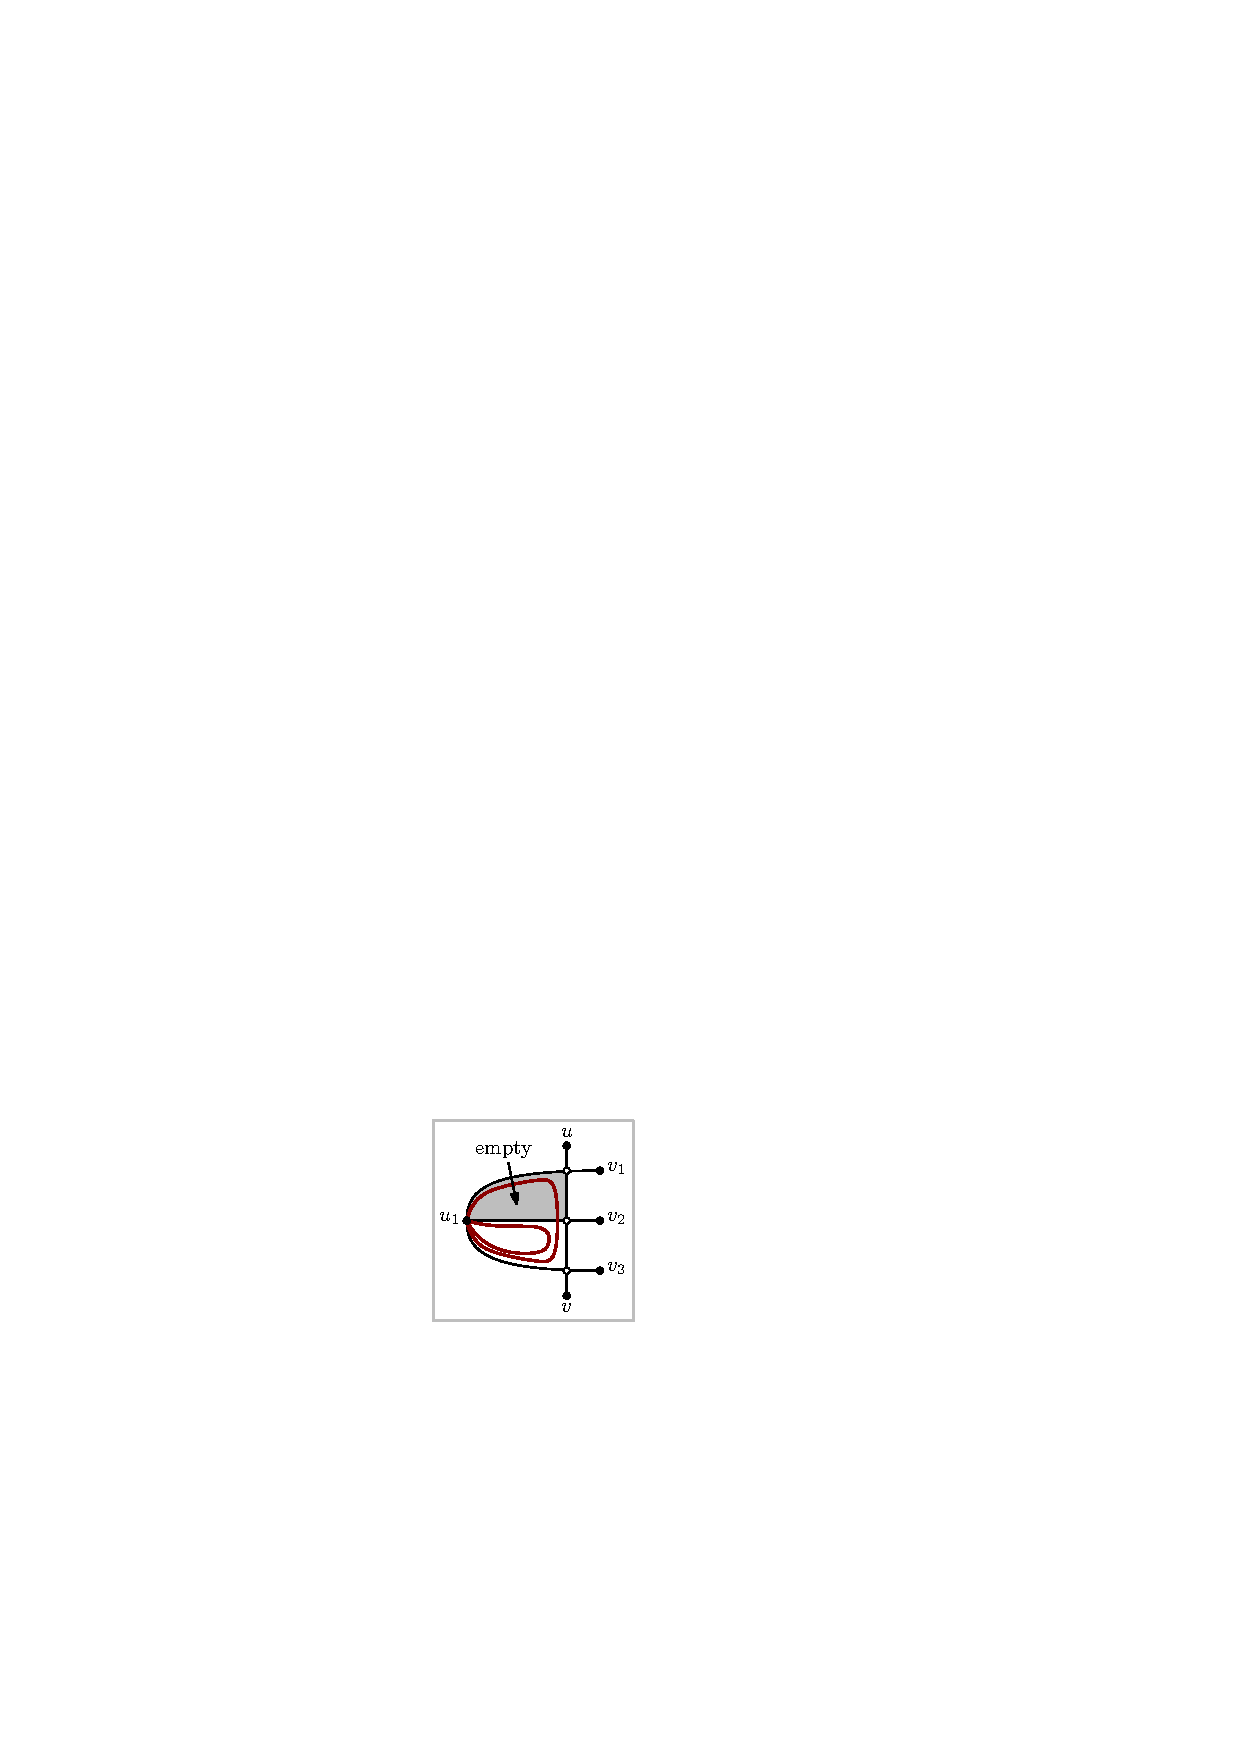
\includegraphics[width=\textwidth,page=1]{images/3planar_small_faces}
        \subcaption{~}\label{fig:3_planar_small_faces_example}
    \end{minipage}
    \begin{minipage}[b]{.24\textwidth}
        \centering
        \includegraphics[width=\textwidth,page=2]{images/3planar_small_faces}
        \subcaption{~}\label{fig:3_planar_small_faces_conf}
    \end{minipage}
    \begin{minipage}[b]{.24\textwidth}
        \centering
        \includegraphics[width=\textwidth,page=3]{images/3planar_small_faces}
        \subcaption{~}\label{fig:3_planar_small_faces_conf_middle_a}
    \end{minipage}
		\begin{minipage}[b]{.24\textwidth}
        \centering
        \includegraphics[width=\textwidth,page=4]{images/3planar_small_faces}
        \subcaption{~}\label{fig:3_planar_small_faces_conf_middle_b}
    \end{minipage}
    \caption{%
    (a):~If the parallel edge $[u_1,u_1]$ is a\pe for edges $(u_2,v_2)$ and $(u_3,v_3)$ then it is also a \pe for edges $(u_1,v_1)$ and $(u_3,v_3)$.  (b)-(d):~Configuration of Lemma~\ref{lem:3_planar_small_faces}.}
    \label{fig:3_planar_small_faces}
\end{figure}

By Lemma~\ref{lem:3_planar_small_faces}, we have that any edge of $G$ that is crossed three times in $\Gamma(G)$ is a chord of a true-planar $k$-cycle (without vertices in its interior) for $6\leq k\leq9$. So, it remains to consider edges of $G$ that have at most two crossings in $\Gamma(G)$, i.e. propagated sets of crossing edges where every edge has at most two crossings. Note that we can not use directly  Lemma~\ref{lem:2_planar_small_faces}, since its proof is based on the fact that optimal $2$-planar graphs have at most $5n-10$ edges, however, we can formulate its analogue lemma as follows:
\begin{lemma}
Let $\Gamma(G)$ be an almost-simple PMCM $3$-planar drawing of an optimal $3$-planar graph $G$ on $n$ vertices. Let $S$ be a propagated set of crossing edges where every edge has at most two crossings. Then edges of $S$ are chords of a true-planar $5$-cycle in $\Gamma(G)$, that contains no vertices in its interior. 
\label{lem:3_planar_small_faces_2}
\end{lemma}
\begin{proof}
We distinguish two cases depending on whether $S$ contains an edge with two crossings or not. Suppose first that this is not the case. Then all edges of $S$ have at most one crossing. Let $e\in S$ crossing with $e'\in S$. Clearly $S=\left\{e,e'\right\}$. The four endpoints of edges $e$ and $e'$ define a \pp $\mathcal{P}$ on $4$ vertices, as in Figure~\ref{fig:3_planar_one_crossing_before} and there are no other edges passing through the \pr $\mathcal{R}$ of $\mathcal{P}$. We proceed by removing edges $e$ and $e'$ and replace them with the $3$-planar pattern of Figure~\ref{fig:3_planar_one_crossing_after}. The derived graph $G'$ has $n'=n+1$ vertices and $m'=m-2+8$ edges, where $n$ and $m$ are the number of vertices and edges of $G$ respectively. Then, $G'$ is $3$-planar and has $m'=5.5n'-10.5>5.5n'-11$ edges; a contradiction.

Now, assume that there exists an edge $e\in S$, where $e=(u,v)$ crossing with two edges $e_1=(u_1,v_1)$ and $e_2=(u_2,v_2)$. By Lemma~\ref{lem:3_planar_independent} edges $e_1$ and $e_2$ are not independent edges. Following the proof of Lemma~\ref{lem:2_planar_small_faces} we can find:
\begin{enumerate}
\item  a \pp on five vertices whose boundary edges define a true planar $5$-cycle with $e$ as a chord, or,
\item a \pp $\mathcal{P}$ on six vertices with at most $6$ edges passing through its \pr  $\mathcal{R}$. In this case, we remove all edges that pass through $\mathcal{R}$ and use the $3$-planar pattern of Figure~\ref{fig:3_planar_polygon_conf_6} that gives $8$ edges in $\mathcal{R}$. The derived graph clearly has more edges than $G$, contradicting its optimality.
\end{enumerate}
\qed
\end{proof}

\begin{figure}[htb]
    \centering
    \begin{minipage}[b]{.24\textwidth}
        \centering
        
\includegraphics[width=\textwidth,page=1]{images/3planar_one_crossing}
        \subcaption{~}\label{fig:3_planar_one_crossing_before}
    \end{minipage}
    \begin{minipage}[b]{.24\textwidth}
        \centering
        
\includegraphics[width=\textwidth,page=2]{images/3planar_one_crossing}
        \subcaption{~}\label{fig:3_planar_one_crossing_after}
    \end{minipage}
		\begin{minipage}[b]{.24\textwidth}
        \centering
        
\includegraphics[width=\textwidth,page=3]{images/3planar_one_crossing}
        \subcaption{~}\label{fig:3_planar_triangle}
    \end{minipage}
    \caption{%
    (a)-(b):~Configurations used in Lemma~\ref{lem:3_planar_small_faces_2}. (c):~Configuration used in Lemma~\ref{lem:3_planar_triangle}}.
    \label{fig:3_planar_one_crossing_1}
\end{figure}

\begin{lemma}
Let $\Gamma(G)$ be an almost-simple PMCM $3$-planar drawing of an optimal $3$-planar graph $G$ on $n$ vertices. There is no true planar $3$-cycle without vertices in its interior. 
\label{lem:3_planar_triangle}
\end{lemma}
\begin{proof}
Suppose that there exists a true planar $3$-cycle in $\Gamma(G)$ without vertices in its interior. Then we can add a vertex in the interior of this cycle, and $6$ edges by using the $3$-planar pattern of Figure~\ref{fig:3_planar_triangle}. The derived graph $G'$ has $n'=n+1$ vertices and $m'=m+6$ edges, where $n$ and $m$ are the number of vertices and edges of $G$ respectively. Then, $G'$ is $3$-planar and has $m'=5.5n'-10.5>5.5n'-11$ edges; a contradiction.
\qed
\end{proof}


By combining Lemmas~\ref{lem:3_planar_small_faces}, \ref{lem:3_planar_small_faces_2} and \ref{lem:3_planar_triangle} the following is straightforward:
 
\begin{corollary}\label{cor:3_planar_faces_general}
The true planar structure $\Pi(G)$ of an almost-simple PMCM $3$-planar drawing of an optimal $3$-planar graph $G$ on $n$ vertices contains faces of length at least $5$ and at most $9$.
\end{corollary}

 
 Now we are ready to prove the main property of almost-simple PMCM $3$-planar drawings of optimal $3$-planar graphs.
 
 \begin{lemma}\label{lem:3_planar_faces_final}
  The true planar structure $\Pi(G)$ of an almost-simple PMCM $3$-planar drawing of an optimal $3$-planar graph $G$ on $n$ vertices contains only faces of length $6$.
 \end{lemma}

 \begin{proof}
  Let $e_{TP}$ be the total number of true planar edges of $G$. By Euler's formula we have that
  
  \begin{equation}
   e_{TP}+2=n+f
  \end{equation}
  
  where $f$ is the total number of faces of $G_{TP}$. Let $s_i$ be the number of faces of $G_{TP}$ of length $i$. By Corollary~\ref{cor:3_planar_faces_general} we have that $5\leq i\leq 9$. Hence,
  
  \begin{equation}
   f=s_5+s_6+s_7+s_8+s_9
  \end{equation}

  Also, by counting the edges of all faces of $G_{TP}$ we have that
  
  \begin{equation}
   2e_{T}=5s_5+6s_6+7s_7+8s_8+9s_9
  \end{equation}

  On the other hand for the number of crossing edges of $G$, say $e_{CR}$, by Lemmas~\ref{lem:3_planar_true_planar} and \ref{lem:3_planar_small_faces_2} we have
  
  \begin{equation}
   e_{CR}=5s_5+8s_6+9s_7+11s_8+14s_9
  \end{equation}

  Hence, for the total number of edges of $G$ we have 
	%\todo{rewrite the equations}
  

  $\begin{array}{ll}
   |E(G)|= & 5.5n-11\\
    \Rightarrow &e_{TP}+e_{CR}= 5.5n-11\\
    \Rightarrow &e_{TP}+e_{CR}= 5.5(e_{TP}-f)\\
    \Rightarrow &2e_{CR}= 9e_{TP}-11f\\
    \Rightarrow &10s_5+16s_6+18s_7+22s_8+28s_9 = 4.5(5s_5+6s_6+7s_7+8s_8+9s_9)\\
   &-11(s_5+s_6+s_7+s_8+s_9)\\
    \Rightarrow &10s_5+16s_6+18s_7+22s_8+28s_9=11s_5+16s_6+20.5s_7+25s_829.5s_9\\
    \Rightarrow &0= s_5+2.5s_7+3s_8+1.5s_9\\
   \Rightarrow &0=s_5=s_7=s_8=s_9
  \end{array}$

The last equation implies that there are only faces of length $6$, hence $f=f_6$.
 \end{proof}

Recall that at the beginning of this section we made the assumption that $\Gamma(G)$ is almost-simple, i.e. there is no pair of edges that cross twice in the drawing $\Gamma(G)$. In the following, we prove that in any PMCM drawing of an optimal $3$-planar graph $G$ on $n$ vertices there are no such pairs of edges.
 %By Lemma~\ref{lem:2_planar_faces} we can characterize all maximal $2$-planar graphs. Since the true planar subgraph of such a graph contains only faces of length $5$, we can start with a $5$-tiling of the plane. Now in the interior of every face of length $5$, we can add all  $5$ missing edges.

\begin{lemma}
Let $\Gamma(G)$ be a PMCM $3$-planar drawing of an optimal $3$-planar graph $G$ on $n$ vertices. Then $\Gamma(G)$ is almost-simple.
%There is no pair of edges that cross twice in $\Gamma(G)$. 
\label{lem:3_planar_cross_twice}
\end{lemma}

\begin{proof}
For a proof by contradiction, suppose that there exist edges $(u_1,v_1)$ and $(u_2,v_2)$ that cross twice at crossing points $c_1$ and $c_2$ as in Figure~\ref{fig:3_planar_cross_twice_general}. Consider the bounded region $\mathcal{R}_{IN}$ defined by $(c_1,c_2)$ segment of edges $(u_1,v_1)$ and $(u_2,v_2)$. Let $V_{IN}\subset V(G)$ be the subset of vertices of $G$ that lie in the interior of $\mathcal{R}_{IN}$. By Lemma~\ref{lem:crossing_twice} $|V_{IN}|\geq 1$. Also, since edges $(u_1,v_1)$ and $(u_2,v_2)$ have already two crossings, there exist at most one edge $e'_1$ and an edge $e'_2$ that cross with $(u_1,v_1)$ and $(u_2,v_2)$ respectively. Since $G$ is connected \todo{mention that G is connected} at least one of $e'_1$ or $e'_2$ has an endpoint in $V_{IN}$. Suppose w.l.o.g. that $e'_1$ is an edge incident to vertex $w$, where $w\in V_{IN}$. Note that vertices $u_1$-$u_2$ define a corner pair of vertices and therefore the corner edge $[u_1,u_2]$ is a \pe (refer to the upper red edge of Figure~\ref{fig:3_planar_cross_twice_region}). Also, since $V_{IN}$ is not empty, another \pe $[u_1,u_2]$ exists (refer to the lower red edge of Figure~\ref{fig:3_planar_cross_twice_region}), such that the bounded region defined by these two \pes contains only $V_{IN}$ in its interior. Let $E_w$ be the set of edges of $G$ that have both endpoints in $V_{IN}$ and cross with edge $e'_1$ in the drawing $\Gamma(G)$ (refer to the light red edge of Figure~\ref{fig:3_planar_cross_twice_region}). Denote by $m_w$ the number of edges in $E_w$. Since $e'_1$ already crosses with edge $(u_1,v_1)$, $m_w\leq 2$. Now we distinguish two cases depending on whether $|V_{IN}|=1$ or $|V_{IN}|\geq 2$.

In the first case, we have that $V_{IN}=\left\{w\right\}$ and edge $E_w$ must be empty, i.e. $m_w=0$. We proceed by removing edges $(u_1,v_1)$, $(u_2,v_2)$ and any other edge that crosses with them, and replace them with the $3$-planar pattern of Figure\ref{fig:3_planar_cross_twice_single}. We add a vertex, say $x$ and true planar edges $(u_1,x)$ and $(x,w)$. Vertices $u_1$, $x$, $w$, $x$, $u_1$, $u_2$ define a \pp $\mathcal{P}$ on six vertices (grey shaded in Figure~\ref{fig:3_planar_cross_twice_single}). In the interior of $\mathcal{P}$ we can add $8$ edges by using the $3$-planar pattern of Figure~\ref{fig:3_planar_polygon_conf_6}. The derived graph, say $G'$, has $n'=n+1$ vertices and at least $m'=m-4+10$ edges, where $n$ and $m$ are the number of vertices and edges of $G$ respectively. Hence $G'$ has $m'\geq 5.5n'-10.5>5.5n'-11$, i.e. more edges than allowed, a clear contradiction.

In the second case, where $|V_{IN}|\geq 2$, we proceed by removing edges $(u_1,v_1)$, $(u_2,v_2)$, any other edge that crosses with them, and edges of $E_w$, i.e. we remove at most $4+m_w$ edges. We replace them with the $3$-planar pattern of Figure\ref{fig:3_planar_cross_twice_main}. We add a vertex, say $x$, true planar edge $(u_1,x)$ and two true planar non homotopic parallel edges $(x,w)$ that contain only vertices $V_{IN}-\left\{w\right\}$ in the bounded region that they define. As in the previous case, vertices $u_1$, $x$, $w$, $x$, $u_1$, $u_2$ define a \pp $\mathcal{P}$ on six vertices (grey shaded in Figure~\ref{fig:3_planar_cross_twice_main}). In the interior of $\mathcal{P}$ we can add $8$ edges by using the $3$-planar pattern of Figure~\ref{fig:3_planar_polygon_conf_6}. Finally, we can add a loop (if it is not already present in $\Gamma(G)$), say $\ell_w$,  at vertex $w$ containing all vertices of $V_{IN}-\left\{w\right\}$ (red loop of Figure~\ref{fig:3_planar_cross_twice_main}). The derived graph, say $G'$, has $n'=n+1$ vertices and at least $m'\geq m-(4+m_w)+11$ edges, where $n$ and $m$ are the number of vertices and edges of $G$ respectively. Hence $G'$ has $m'\geq 5.5n'-9.5-m_w$. Since $G'$ is $3$-planar $m'\leq 5.5n'-11$ also holds. By combining the two equations we have that $5.5n'-9.5-m_w\leq 5.5n'-11\Rightarrow 1.5\leq m_w$. Recall that $m_w\geq 2$, hence it must be the case that $m_w=2$ and $m'= m-(4+m_w)+11$. However, the last equality holds only in the case where the loop $\ell_w$ already exists in $G$. Now, note that any edge of $E_w$ crosses twice with loop $\ell_w$, which implies that $\ell_w$ has at least $4$ crossings, a clear contradiction.
\end{proof}

\begin{figure}[htb]
    \centering
    \begin{minipage}[b]{.24\textwidth}
        \centering
        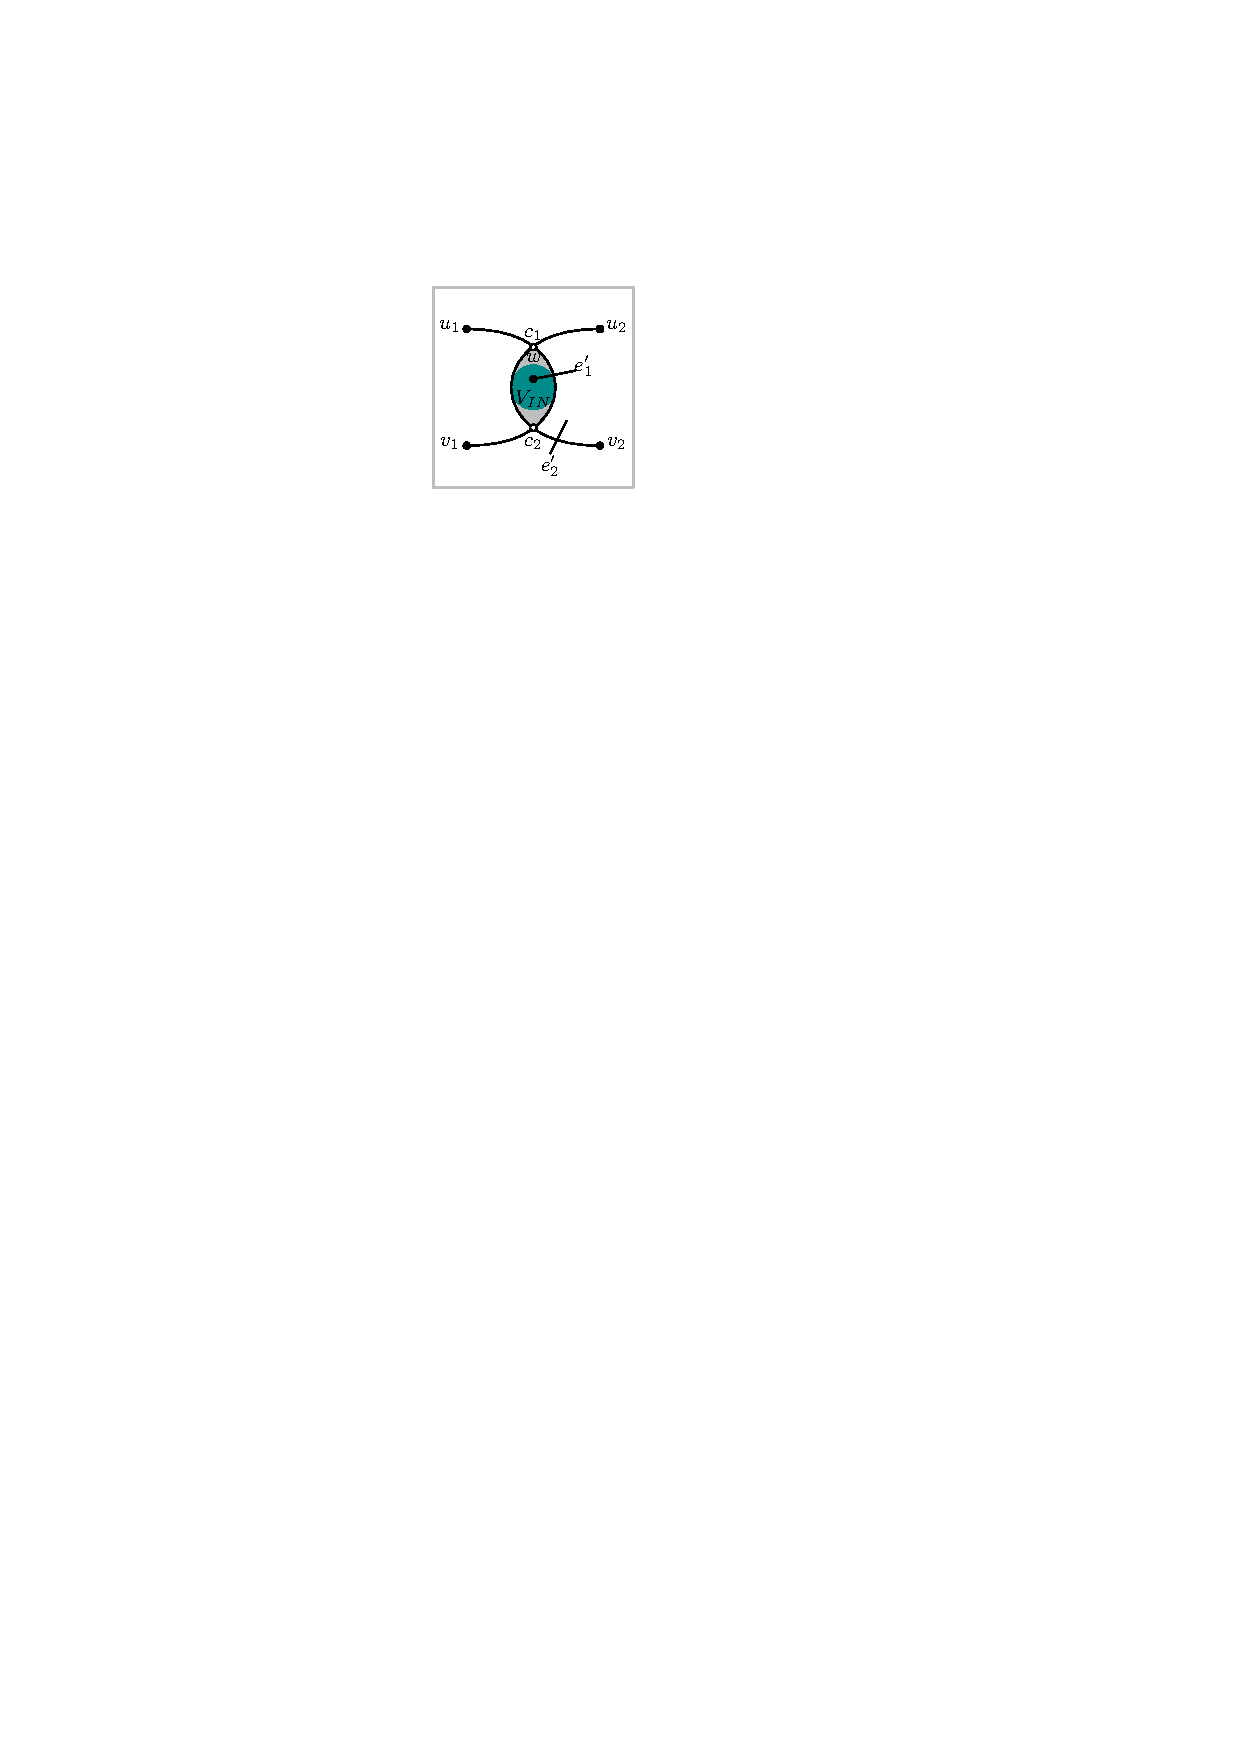
\includegraphics[width=\textwidth,page=1]{images/3_planar_cross_twice}
        \subcaption{~}\label{fig:3_planar_cross_twice_general}
    \end{minipage}
    \begin{minipage}[b]{.24\textwidth}
        \centering
        \includegraphics[width=\textwidth,page=2]{images/3_planar_cross_twice}
        \subcaption{~}\label{fig:3_planar_cross_twice_region}
    \end{minipage}
		\begin{minipage}[b]{.24\textwidth}
        \centering
        \includegraphics[width=\textwidth,page=3]{images/3_planar_cross_twice}
        \subcaption{~}\label{fig:3_planar_cross_twice_single}
    \end{minipage}
    \begin{minipage}[b]{.24\textwidth}
        \centering
        \includegraphics[width=\textwidth,page=4]{images/3_planar_cross_twice}
        \subcaption{~}\label{fig:3_planar_cross_twice_main}
    \end{minipage}
    \caption{%
    (a)-(d):~Configurations used in Lemma~\ref{lem:3_planar_cross_twice}.
    \label{fig:3_planar_one_crossing_2}}
\end{figure}

By combining Lemmas~\ref{lem:3_planar_faces_final} and \ref{lem:3_planar_cross_twice}, we can characterize all optimal $3$-planar graphs:


 By Lemma~\ref{lem:3_planar_cross_twice} we have that Lemma~\ref{lem:3_planar_faces_final} holds for all maximal $3$-planar graphs. Since the true planar subgraph of such a graph contains only faces of length $6$, we can start with a $6$-tiling of the plane\todo{rephrase}. Now in the interior of every face of length $6$, we can add all  $8$ missing edges using the $3$-planar pattern of Figure~\ref{fig:3_planar_polygon_conf_6}.
 %By Lemma~\ref{lem:3_planar_faces_final} we can characterize all maximal $3$-planar graphs. Since the true planar subgraph of such a graph contains only faces of length $6$, we can start with a $6$-tiling of the plane. Now in the interior of every face of length $6$, we can add all  $8$ missing edges.

